\documentclass[11pt]{article}

\usepackage[margin=1in]{geometry}
\usepackage[T1]{fontenc}
\usepackage[utf8]{inputenc}
\usepackage{lmodern}
\usepackage{microtype}
\usepackage{amsmath,amssymb,amsfonts}
\usepackage{bm}
\usepackage{booktabs}
\usepackage{multirow}
\usepackage{array}
\usepackage{graphicx}
\usepackage{subcaption}
\usepackage{float}
\usepackage{url}
\usepackage{xcolor}
\usepackage{hyperref}
\usepackage[nameinlink,noabbrev]{cleveref}
\usepackage{enumitem}
\usepackage{longtable}
\usepackage{tabularx}
\usepackage{makecell}
\usepackage{setspace}
\usepackage{authblk}
\usepackage[numbers,sort&compress]{natbib}
\usepackage{pdflscape}
\usepackage[section]{placeins}

\hypersetup{
  colorlinks=true,
  linkcolor=blue!60!black,
  citecolor=blue!60!black,
  urlcolor=blue!60!black,
  pdftitle={Intellitons: Quasiparticle Structure in Large Language Models},
  pdfauthor={}
}

\title{Intellitons: Quasiparticles of Computation in Large Language Models\\
\large A Field-Theoretic Framework for Real-Time Hallucination Detection and Internal Dynamics}

\author[1]{Zhaoping Xiong\thanks{xiongzhp150@gmail.com}}
\affil[1]{ProtonUnfold Tech. Co. Ltd}
\date{\today}

\begin{document}
\maketitle

\begin{abstract}
We introduce \emph{Intellitons}, a novel conceptual and operational framework that models the internal representations of large language models (LLMs) as recurrent collective excitation modes within a discrete token-layer lattice field. By applying techniques inspired by lattice gauge theory and effective field theory, we extract quasiparticle-like observables---such as pole masses, lattice dispersion relations, helicity, and renormalization-group flow---from the residual stream dynamics of transformer architectures. Our central finding is that this physical analogy provides a powerful, low-dimensional coordinate system for tracking the stability of model generation. Specifically, we demonstrate that grounded, factual generation corresponds to the robust occupation of a dominant, stable Intelliton sector. In contrast, hallucination-prone generation is characterized by measurable spectral divergence, coherence loss, and displacement from this grounded sector. This separation enables a critical application: the real-time detection and post-generation diagnosis of hallucinations based purely on internal dynamical stability, without relying on external reference models or confidence heuristics. While we validate this framework across multiple architectures (including Qwen and Mistral families) to show how scaling and instruction tuning compress or fragment the excitation landscape, the primary contribution of this work is establishing Intelliton dynamics as a principled, mechanistic signal for monitoring the faithfulness of LLM reasoning.
\end{abstract}

\section{Introduction}
Large language models (LLMs) have demonstrated remarkable capabilities across diverse cognitive tasks, yet their internal computational mechanisms remain notoriously opaque \citep{bommasani2021opportunities,bubeck2023sparks}. While mechanistic interpretability has made significant strides by isolating individual neurons, attention heads, and static feature directions \citep{olah2020zoom,elhage2021mathematical,geva2020transformer}, these approaches often struggle to capture the macroscopic, dynamic evolution of information as it propagates through the depth of the network. A fundamental scientific question remains: \emph{what are the effective, collective degrees of freedom that govern the stability and reliability of LLM generation?}

In this paper, we propose a novel perspective inspired by condensed matter physics and quantum field theory \citep{wilson1979problems,weinberg1995quantum,cheung2008effective,kaplan2024simplest}. We model the transformer's residual stream as a discrete field defined on a token-layer lattice, where token positions act as spatial coordinates, layer indices act as an effective time or renormalization scale, and hidden dimensions represent internal degrees of freedom. Within this framework, we hypothesize the existence of \emph{Intellitons}---recurrent, stable collective excitation modes that emerge from the microscopic interactions of the network's parameters. Much like phonons or magnons in physical systems, Intellitons are not fundamental entities, but rather emergent quasiparticle-like structures that provide a compact, low-dimensional summary of complex, high-dimensional dynamics.

We operationalize this concept by extracting effective physical observables from the residual stream, including momentum spectra, pole masses derived from discrete propagators, lattice dispersion relations, and renormalization-group (RG) flow parameters \citep{raju2026modelerrors}. By cataloging these modes across diverse prompts, we construct an ``Intelliton spectrum'' for a given model.

Crucially, this physical analogy is not merely descriptive; it yields a powerful diagnostic tool for one of the most pressing challenges in LLM deployment: hallucination \citep{ji2023survey,huang2023survey}. Traditional hallucination detection often relies on external verification, self-consistency sampling, or output probability heuristics \citep{manakul2023selfcheckgpt,kadavath2022language}. In contrast, the Intelliton framework allows us to view hallucination as an internal dynamical instability. We demonstrate that grounded, factual generation corresponds to the robust occupation of a dominant, stable Intelliton sector. When a model hallucinates, its internal trajectory exhibits measurable spectral divergence, coherence loss, and displacement from this grounded sector. This enables the use of Intelliton observables as real-time, generation-time warning signals for unfaithful reasoning.

\paragraph{Main Contributions.}
Our work introduces the Intelliton framework and validates its utility through extensive experiments across multiple architectures (Qwen3 and Mistral families). Our primary contributions are:
\begin{enumerate}[leftmargin=1.5em]
    \item \textbf{The Intelliton Framework:} We formalize the extraction of quasiparticle-like observables from transformer residual streams, providing a novel, physics-inspired coordinate system for LLM interpretability.
    \item \textbf{Real-Time Hallucination Detection:} We establish that hallucination-prone generation occupies a distinct, weaker dynamical regime compared to grounded factual generation, enabling real-time monitoring of generation stability based purely on internal state trajectories.
    \item \textbf{Architectural and Alignment Insights:} By comparing base vs. instruct models and scaling from 4B to 8B parameters, we show that instruction tuning compresses the internal excitation landscape, while parameter scaling strengthens the dominant grounded sectors. Furthermore, cross-family comparisons reveal that different architectures (e.g., Qwen vs. Mistral) exhibit fundamentally different degrees of spectral fragmentation.
\end{enumerate}

\section{Related Work and Conceptual Framing}
This work sits at the intersection of mechanistic interpretability, spectral analysis of neural activations, and effective descriptions of large-scale computation \citep{olah2020zoom,elhage2021mathematical}. The closest conceptual analogy is not to fundamental particle physics, but to condensed matter and effective field theory, where coarse-grained degrees of freedom summarize complex microscopic interactions \citep{wilson1979problems,weinberg1995quantum}. In our case, singular modes of the residual field act as these coarse-grained units, and their stability across depth and prompts motivates the quasiparticle terminology.

A key distinction from many interpretability approaches is our explicit emphasis on \emph{dynamics}. Intellitons are not merely static feature directions; they are tracked across layers and during generation. This permits a unified description of discovery, characterization, and downstream applications such as hallucination diagnostics.

\section{Methodology}
\subsection{The Residual Stream as a Token-Layer Lattice Field}
Given a residual tensor $\phi[l,t,d]$, where $l$ indexes the layer, $t$ indexes the token position, and $d$ indexes the hidden channel, we treat the model state as a discrete field on a one-dimensional token lattice evolving across depth. This construction is inspired by the broader use of representation geometry and activation-space structure in transformer analysis \citep{voita2023neural,belrose2023leace}.

For each prompt category, our computational pipeline performs the following operations:
\begin{enumerate}[leftmargin=1.5em]
    \item Extracts residual streams and attention maps during forward passes.
    \item Computes token-space Fourier spectra to analyze spatial frequencies.
    \item Performs layer-wise singular value decomposition (SVD) to isolate dominant modes.
    \item Computes propagator-based pole masses and lattice masses.
    \item Estimates dispersion relations and helicity-like diagnostics.
    \item Computes effective field theory (EFT) and renormalization-group (RG) summaries.
    \item Merges recurrent modes into a discrete Intelliton species catalog.
    \item Tracks species occupations dynamically during autoregressive generation.
\end{enumerate}

\subsection{Operational Definition of an Intelliton}
We define an Intelliton as a mode that is:
\begin{itemize}[leftmargin=1.5em]
    \item Spectrally dominant and recurrent across diverse prompts.
    \item Trackable across layers via mode matching (e.g., cosine similarity of singular vectors).
    \item Describable by effective observables such as mass, momentum, spin-like entropy score, helicity, and wavefunction renormalization.
    \item Sufficiently stable to support cross-prompt merging into a unified species-level catalog.
\end{itemize}

We construct the Intelliton catalog by aggregating modes that exhibit high similarity across contexts, assigning species identifiers ($I_0, I_1, \dots$) and computing their aggregate effective quantities.

\subsection{Propagator, Dispersion, and RG Diagnostics}
Let $\sigma_l^{(i)}$ denote the singular value of mode $i$ at layer $l$. The pipeline constructs normalized depth-direction curves and computes a spectral function via a discrete Fourier transform over depth, from which a pole-like mass estimate is extracted. Independently, a lattice mass is estimated from momentum-dependent evolution using a discrete dispersion relation. An EFT module then computes running masses, fixed-point layers, anomalous dimensions, and wavefunction renormalization factors $Z$. This use of effective observables is methodologically aligned with coarse-grained descriptions that seek low-dimensional summaries of high-dimensional model behavior \citep{raju2026modelerrors}.

\subsection{Generation-Time Dynamics and Hallucination Diagnostics}
To analyze generation-time dynamics, we project autoregressive states onto the established species vectors to estimate occupations and mode activation shifts over time. We compare grounded and hallucination-prone prompts through spectral divergence, coherence loss, entropy gap, and mode stability. This yields a dynamic interpretation of hallucination as an instability, weakening, or displacement from grounded Intelliton sectors.

\section{Experimental Setup}
We evaluate our framework across five distinct LLMs to assess the impact of scale, alignment, and architectural family:
\begin{itemize}[leftmargin=1.5em]
    \item \texttt{Qwen3-4B-Base} and \texttt{Qwen3-8B-Base}
    \item \texttt{Qwen3-4B} and \texttt{Qwen3-8B} (Instruct-tuned)
    \item \texttt{Mistral-7B-v0.3}
\end{itemize}

We utilize a diverse set of prompt categories---including arithmetic, factual recall, logical reasoning, pronoun tracking, and syntactic agreement---to stimulate different cognitive circuits. For our primary analysis, we fix the context window to 128 tokens and retain the top 20 singular modes per layer.

\section{Results}
\subsection{Intelliton Spectrum of Qwen3-4B-Base}
The \texttt{Qwen3-4B-Base} model provides the clearest single demonstration of the Intelliton framework. As detailed in \Cref{fig:appendix-qwen4bbase-catalog}, the model yields a remarkably compact catalog of exactly \textbf{6 species}. The dominant species, $I_0$, exhibits a spin-like score of 1.84, a pole mass of 0.1275, a lattice mass of 0.0083, and an amplitude of 6167.1. It is active across arithmetic, factual recall, and logical reasoning tasks. In contrast, the remaining species ($I_1$ through $I_5$) are weaker but highly task-linked, clustering around fixed-point layer 13 with infrared (IR) classification.

This structure suggests a two-level organization: a strong, shared backbone excitation alongside several smaller, specialized species. Furthermore, the dominant species peaks at momentum $k \approx \pi$, while the remaining species cluster at $k \approx 0$, indicating the coexistence of high-frequency and low-frequency structures on the token lattice. The renormalization-group (RG) flow, illustrated in \Cref{fig:qwen4bbase-rg}, highlights a mid-layer reorganization where the dominant mode remains crossover-like while secondary species settle into stable IR-like behavior.

\begin{figure}[H]
    \centering
    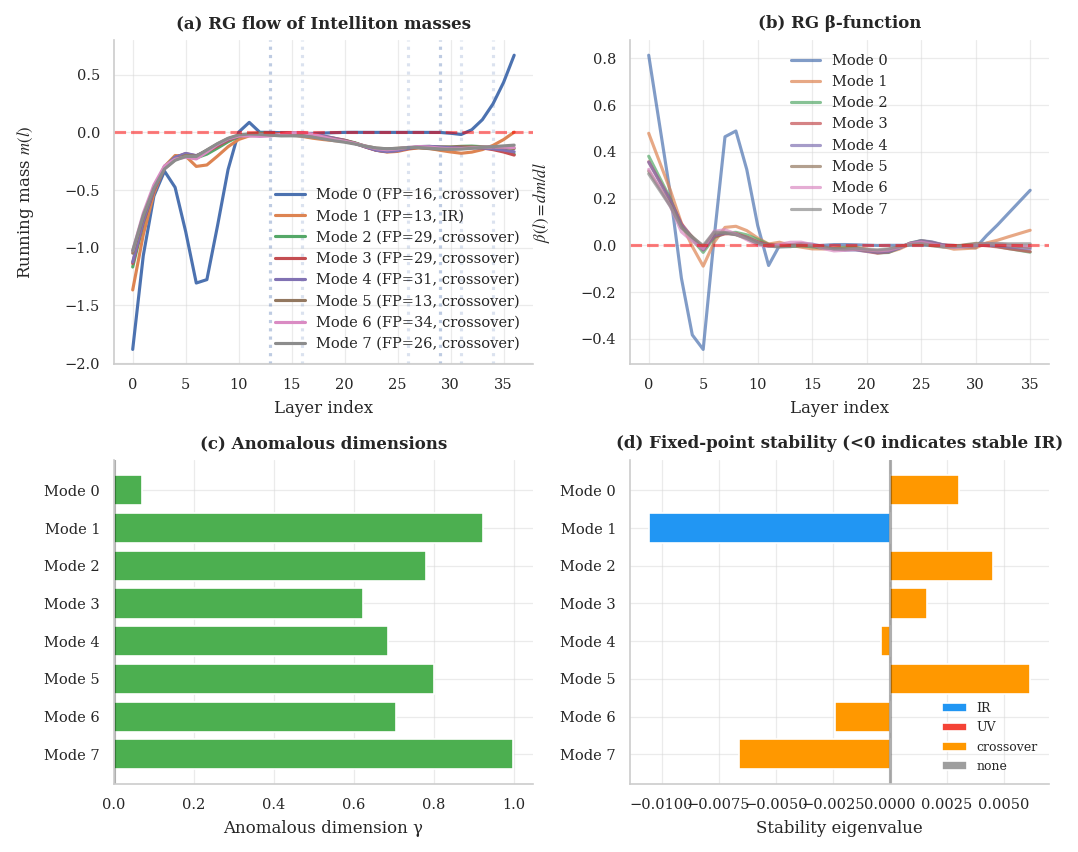
\includegraphics[width=\textwidth]{results_paper/Qwen3-4B-Base/rg_flow.png}
    \caption{Main-text RG-flow summary of the \texttt{Qwen3-4B-Base} case. The mid-layer reorganization shows the dominant mode remaining crossover-like while secondary species settle into more IR-like behavior.}
    \label{fig:qwen4bbase-rg}
\end{figure}

\subsection{Dynamical Stability and Hallucination Detection}
For \texttt{Qwen3-4B-Base}, grounded factual prompts exhibit markedly stronger generation-time Intelliton activation than hallucination-prone prompts. Over the first eight generation steps, grounded prompts maintain mean mode activation shifts around 0.97--1.37, whereas hallucination-prone prompts remain suppressed around 0.32--0.41. Grounded deviation is near zero by construction for grounded prompts but strongly negative for hallucination-prone prompts (typically around $-9$ to $-11$).

This separation indicates that hallucination is not merely an output-level failure but corresponds to a measurable displacement from the grounded Intelliton sector. Stylistic continuation occupies an intermediate regime, confirming that the metric captures factual groundedness rather than generic fluency.

From an application perspective, this is a critical outcome. The Intelliton framework supports two complementary use cases: \emph{post-generation diagnosis} and \emph{real-time monitoring}. Post-generation, one can compare responses through spectral divergence, coherence loss, and sector displacement, as shown in \Cref{fig:qwen4bbase-hall}. During generation, one can monitor whether the evolving trajectory remains inside a grounded sector or drifts toward a weaker regime, as demonstrated in \Cref{fig:qwen4bbase-traj}. This naturally motivates using Intelliton observables as real-time hallucination warning signals.

\begin{figure}[H]
    \centering
    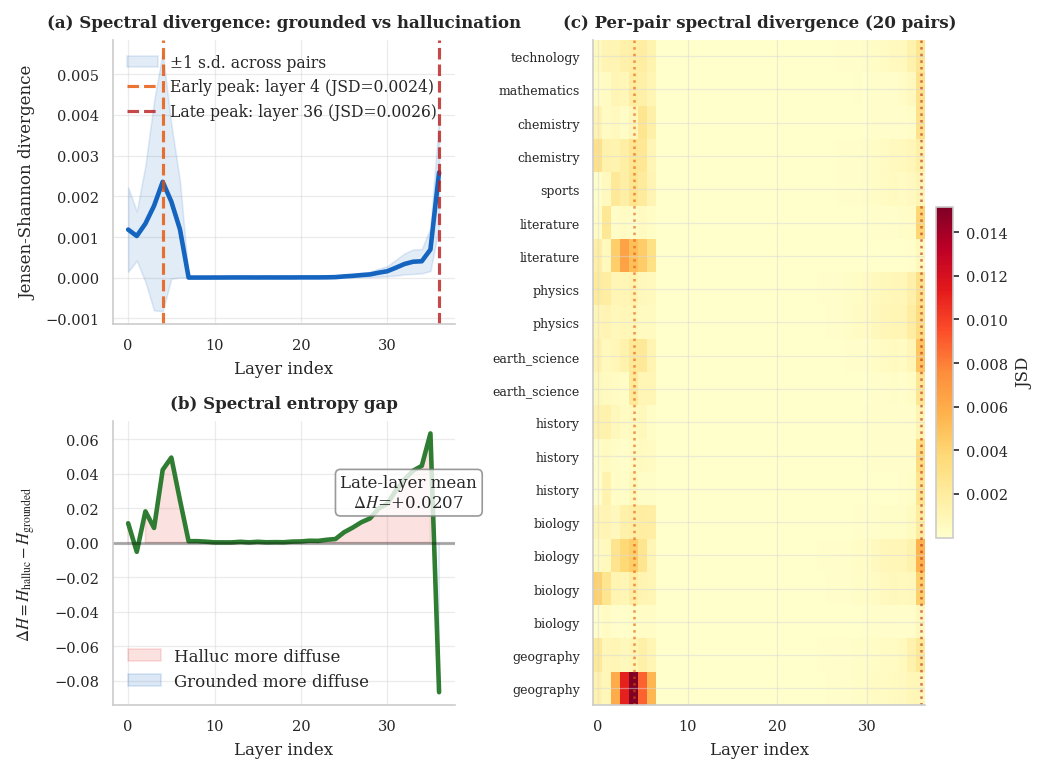
\includegraphics[width=\textwidth]{results_paper/Qwen3-4B-Base/hallucination_diagnostics.png}
    \caption{Hallucination diagnostics for \texttt{Qwen3-4B-Base}. Grounded and hallucination-prone prompts separate clearly in Intelliton space, supporting the use of spectral divergence and related observables for post-generation hallucination diagnosis.}
    \label{fig:qwen4bbase-hall}
\end{figure}

\begin{figure}[H]
    \centering
    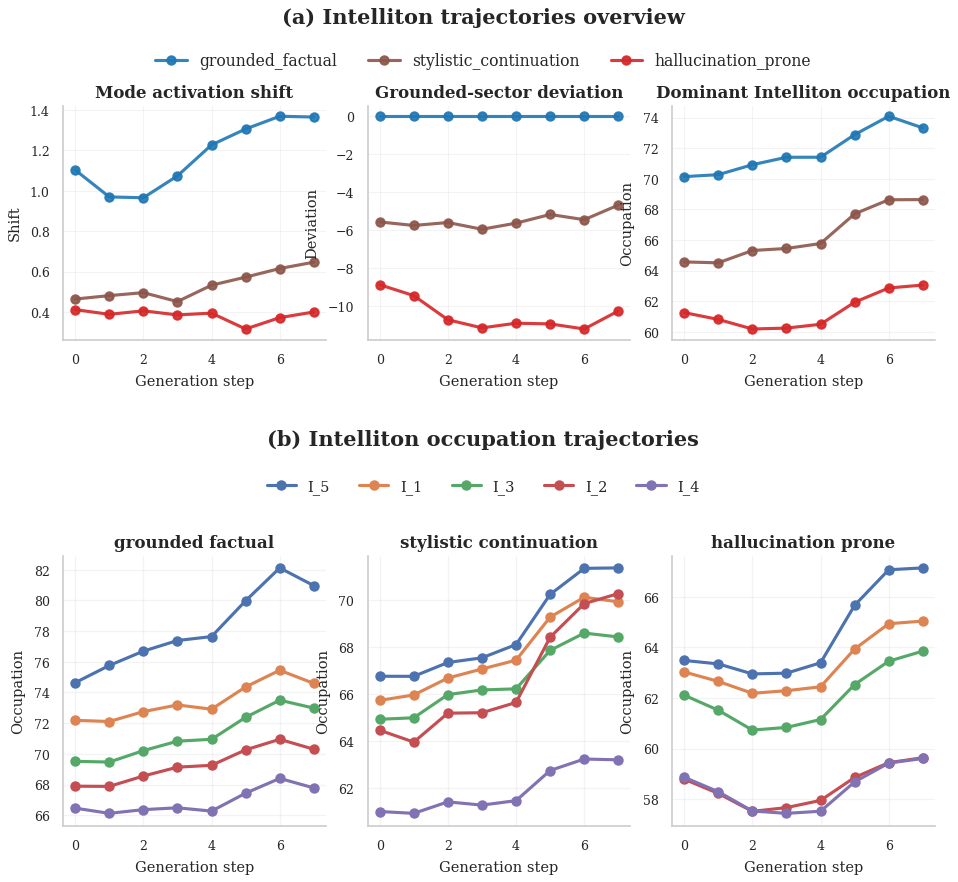
\includegraphics[width=\textwidth]{results_paper/Qwen3-4B-Base/intelliton_trajectory_merged.png}
    \caption{Trajectory diagnostics for \texttt{Qwen3-4B-Base}. Grounded prompts exhibit stronger activation shifts and higher dominant occupations than hallucination-prone prompts, indicating that Intelliton trajectories may also support real-time hallucination monitoring during generation.}
    \label{fig:qwen4bbase-traj}
\end{figure}

\subsection{Impact of Instruction Tuning on the Excitation Landscape}
Comparing the base and instruct-tuned variants reveals significant structural shifts. Within the Qwen 4B pair, \texttt{Qwen3-4B-Base} yields 6 species whereas \texttt{Qwen3-4B} yields 5 (\Cref{tab:model-summary}). The base model displays a momentum split between a dominant $k \approx \pi$ mode and several $k \approx 0$ modes. In contrast, the instruct model becomes more homogeneous, with all listed species concentrated near momentum 1.885 and all fixed-point types labeled as crossover (\Cref{fig:appendix-qwen4b-catalog}). A similar homogenization occurs in the 8B pair (\Cref{fig:appendix-qwen8b-catalog}).

These results suggest that instruction tuning regularizes or compresses the model's excitation geometry: it preserves the leading backbone mode but reduces diversity in the rest of the spectrum. The effect is also visible in grounded dynamics, where the grounded-mode activation mean drops from 32.68 to 29.13 in the 4B pair and from 60.26 to 57.14 in the 8B pair (\Cref{tab:model-summary}).

The generation-time diagnostics, shown in \Cref{fig:qwen4b-traj-main} and \Cref{fig:qwen8b-traj-main}, demonstrate that while instruct tuning compresses the internal excitation geometry, it does not eliminate the critical separation between grounded and hallucination-prone trajectories.

\begin{figure}[H]
    \centering
    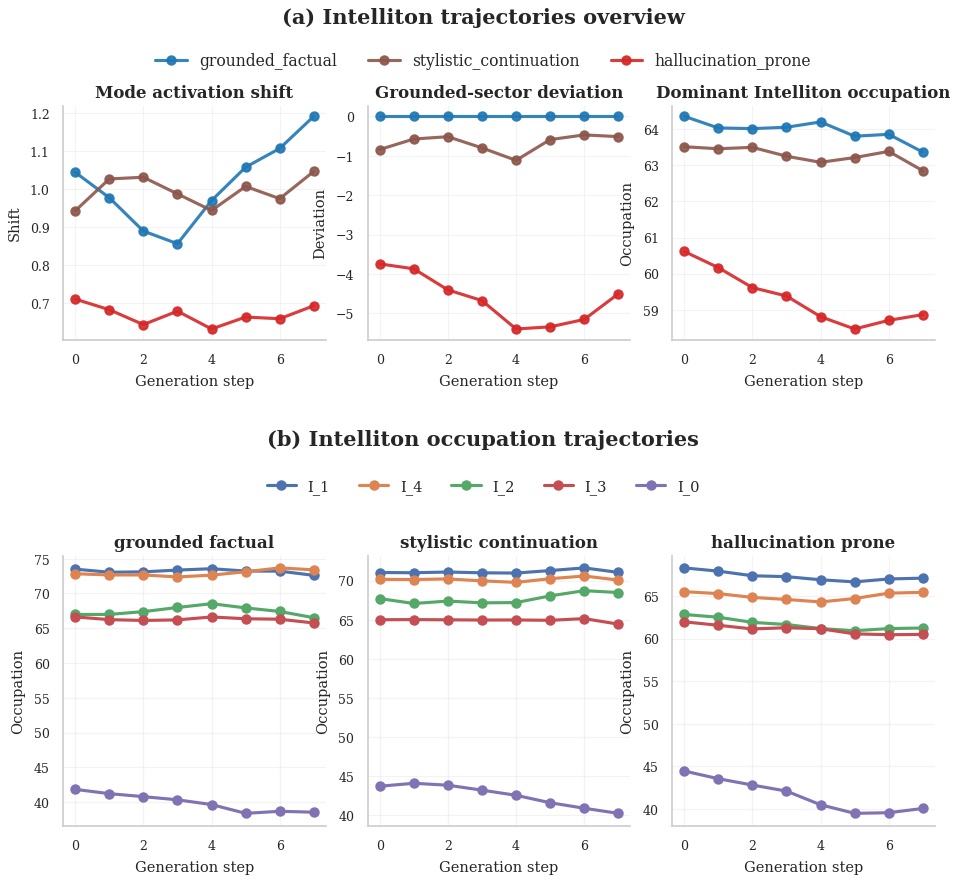
\includegraphics[width=\textwidth]{results_paper/Qwen3-4B/intelliton_trajectory_merged.png}
    \caption{Main-text trajectory diagnostics for \texttt{Qwen3-4B}. The instruct-tuned 4B model retains separation between grounded and hallucination-prone prompt regimes, but with a weaker grounded-sector contrast than the base model.}
    \label{fig:qwen4b-traj-main}
\end{figure}

\begin{figure}[H]
    \centering
    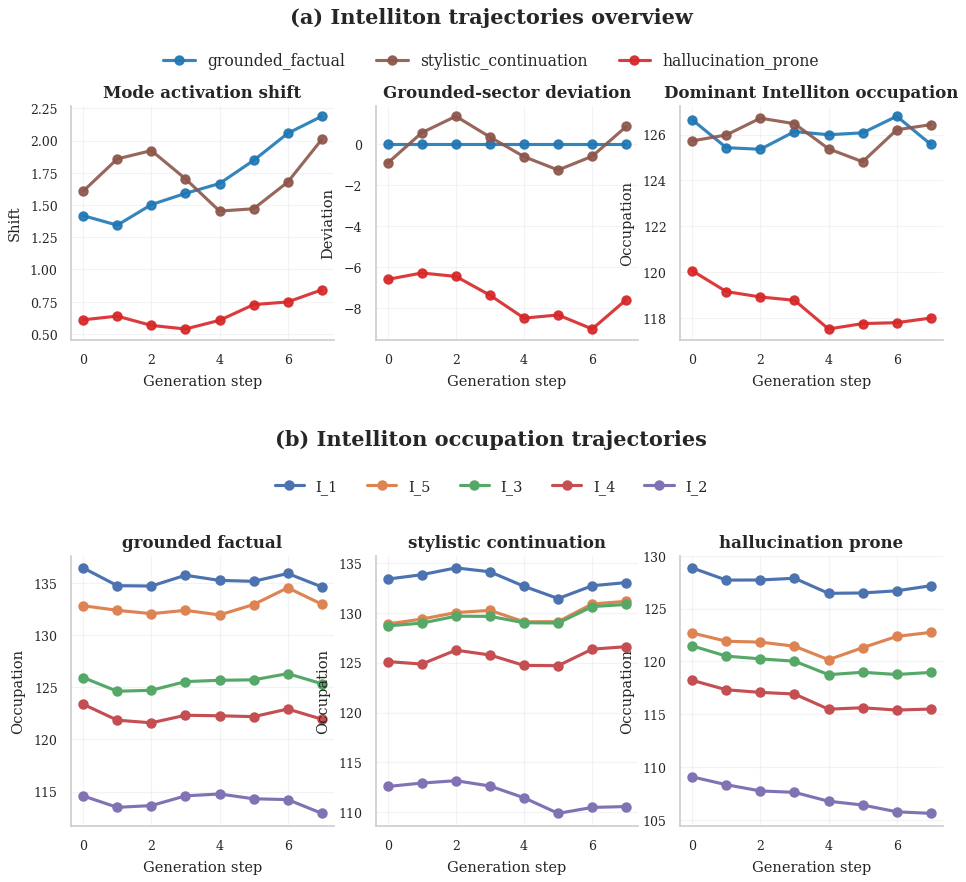
\includegraphics[width=\textwidth]{results_paper/Qwen3-8B/intelliton_trajectory_merged.png}
    \caption{Main-text trajectory diagnostics for \texttt{Qwen3-8B}. Scaling preserves strong grounded-sector dynamics even after instruction tuning.}
    \label{fig:qwen8b-traj-main}
\end{figure}

\subsection{Effects of Parameter Scaling on Grounded Sectors}
Scaling within the Qwen family produces a clear strengthening of dominant internal excitations. As detailed in \Cref{tab:leading-species}, the leading species amplitude rises from 6167.1 in \texttt{Qwen3-4B-Base} to 7908.4 in \texttt{Qwen3-8B-Base}, and the grounded-mode activation mean nearly doubles from 32.68 to 60.26 (\Cref{tab:model-summary}). The instruct pair shows a similar trend.

This indicates that parameter scaling does more than expand capacity in an undifferentiated way. Under the Intelliton view, larger models develop stronger and more sharply occupied grounded sectors, while preserving a compact species-level description (\Cref{fig:appendix-qwen8bbase-catalog}). The RG flow (\Cref{fig:qwen8bbase-rg-main}) and trajectory diagnostics (\Cref{fig:qwen8bbase-traj-main}) provide direct evidence for this strengthened internal organization.

\begin{figure}[H]
    \centering
    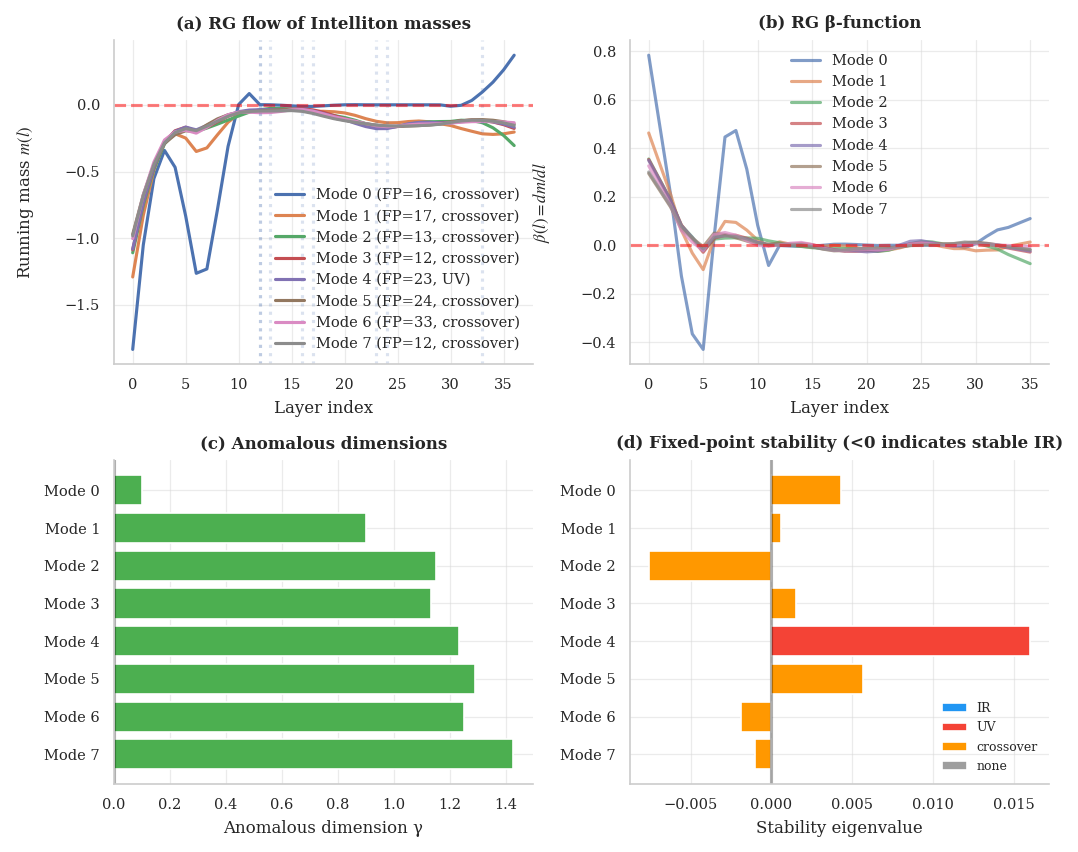
\includegraphics[width=\textwidth]{results_paper/Qwen3-8B-Base/rg_flow.png}
    \caption{Main-text RG-flow diagnostics for \texttt{Qwen3-8B-Base}. Relative to the 4B base model, the 8B base model exhibits a stronger and slightly richer renormalization structure.}
    \label{fig:qwen8bbase-rg-main}
\end{figure}

\begin{figure}[H]
    \centering
    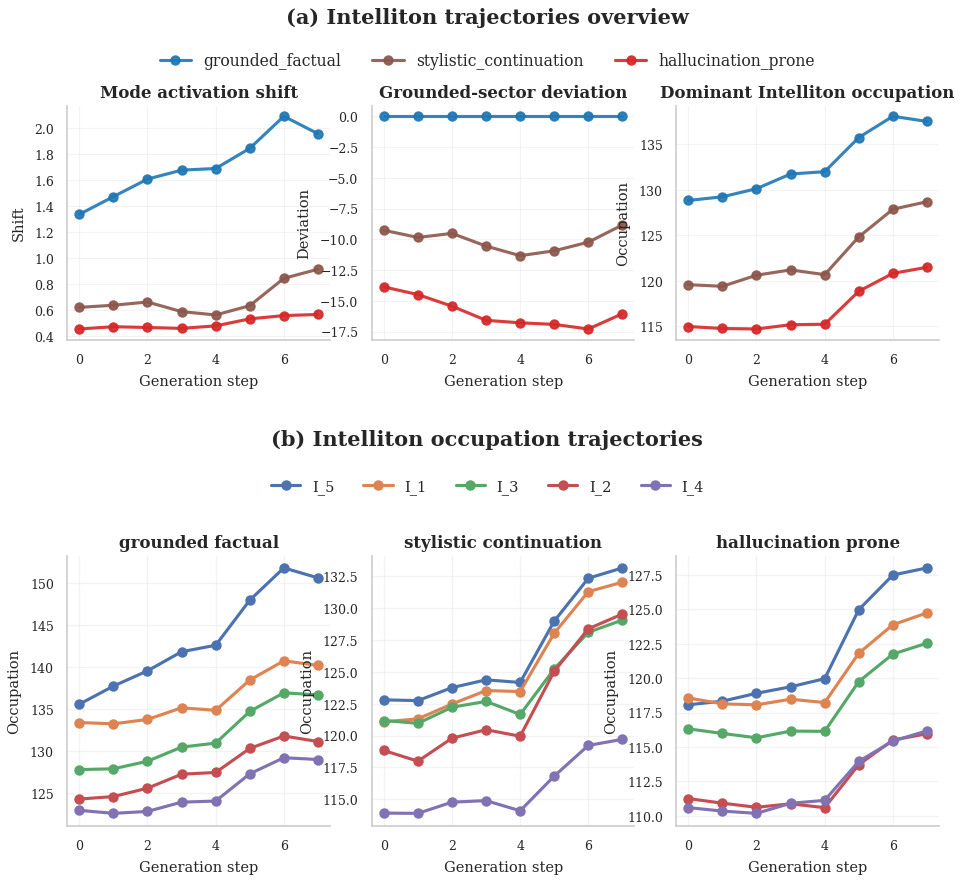
\includegraphics[width=\textwidth]{results_paper/Qwen3-8B-Base/intelliton_trajectory_merged.png}
    \caption{Main-text trajectory diagnostics for \texttt{Qwen3-8B-Base}. Grounded-sector activation is substantially stronger than in the 4B base model, consistent with scale-induced strengthening of dominant Intelliton structure.}
    \label{fig:qwen8bbase-traj-main}
\end{figure}

\subsection{Cross-Architectural Variations in Excitation Spectra}
The cross-family comparison is especially striking. Under the identical analytical pipeline, \texttt{Mistral-7B-v0.3} yields a \textbf{25-species} catalog (\Cref{fig:appendix-mistral-catalog}), far larger than the 5--7 species seen in the Qwen models. Its grounded-mode activation mean is only 21.48, with an unusually large standard deviation of 46.56 (\Cref{tab:model-summary}). Several species are classified as UV-like at late fixed-point layers, in contrast to the more compact and cleaner Qwen spectra.

The broad conclusion is that architectural family strongly affects the granularity and stability of the internal excitation landscape. Qwen appears dominated by a few strong collective modes, whereas Mistral appears more fragmented and spectrally crowded. This is further evidenced by Mistral's RG flow (\Cref{fig:mistral-rg-main}) and highly variable trajectory dynamics (\Cref{fig:mistral-traj-main}).

\begin{figure}[H]
    \centering
    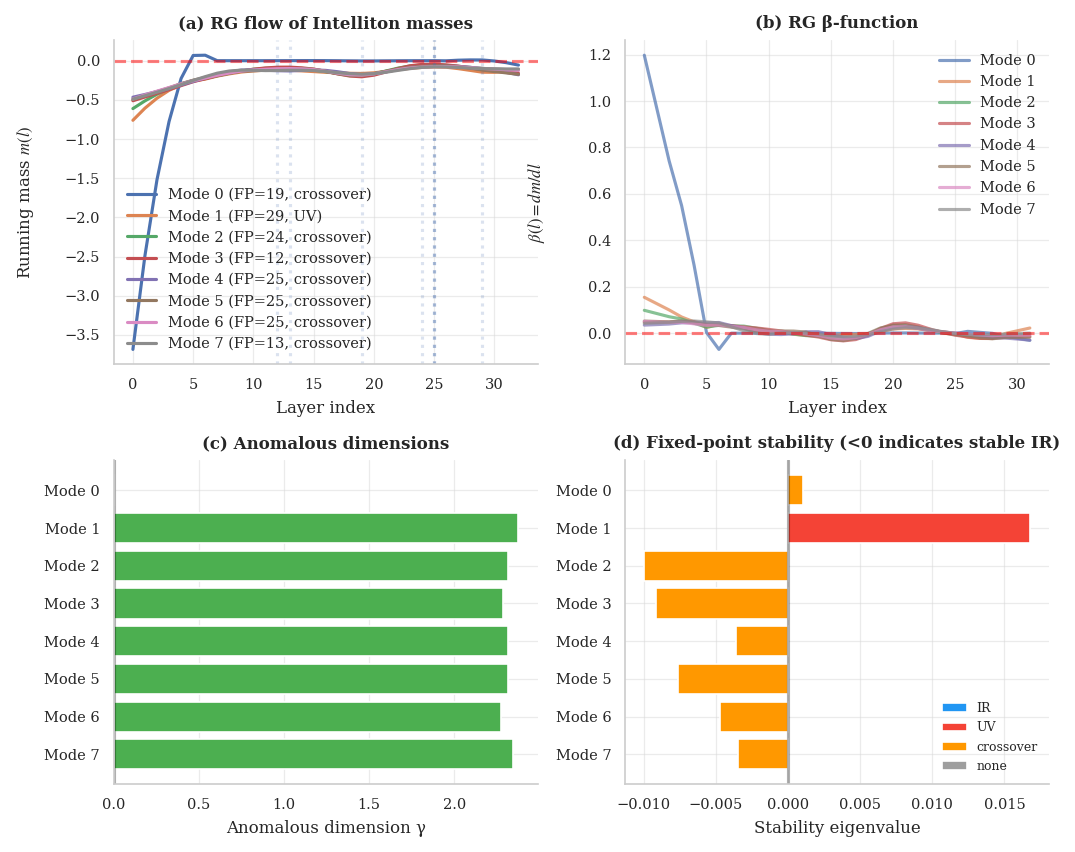
\includegraphics[width=\textwidth]{results_paper/Mistral-7B-v0.3/rg_flow.png}
    \caption{Main-text RG-flow diagnostics for \texttt{Mistral-7B-v0.3}. The family-level contrast with Qwen is visible in a less compact renormalization structure.}
    \label{fig:mistral-rg-main}
\end{figure}

\begin{figure}[H]
    \centering
    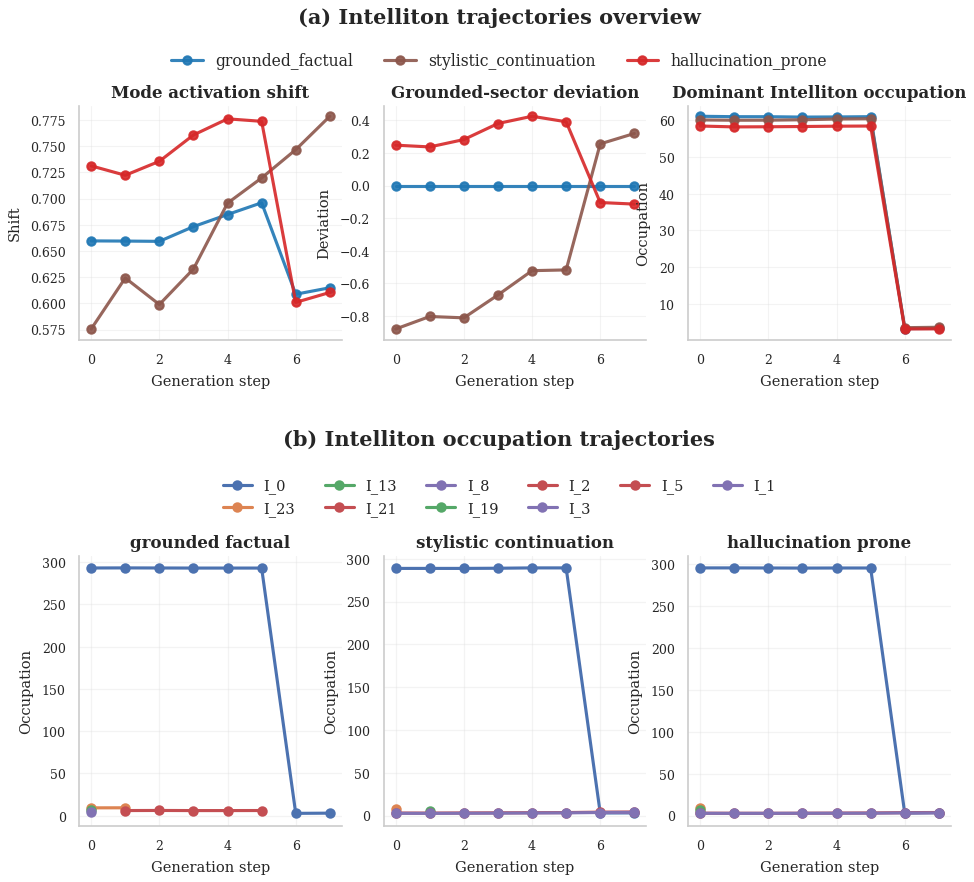
\includegraphics[width=\textwidth]{results_paper/Mistral-7B-v0.3/intelliton_trajectory_merged.png}
    \caption{Main-text trajectory diagnostics for \texttt{Mistral-7B-v0.3}. The broader and noisier trajectory structure is consistent with a more fragmented internal excitation landscape than in the Qwen family.}
    \label{fig:mistral-traj-main}
\end{figure}

\section{Discussion}
Our experiments support the claim that a quasiparticle-like language provides a rigorous, effective description of internal transformer organization. Three aspects are particularly noteworthy.

First, the framework is \emph{compact}. Instead of tracking thousands of unstable latent directions, it produces species catalogs with low cardinality for the Qwen family. Second, the framework is \emph{comparative}. It clearly distinguishes base versus instruct tuning, 4B versus 8B scaling, and Qwen versus Mistral family structures. Third, the framework is \emph{dynamical}. It links internal spectra directly to generation-time behavior, offering a mechanistic lens into hallucination-prone settings.

At the same time, several limitations must be acknowledged. The terminology is physics-inspired and should be understood operationally. The resulting catalog depends on prompt design, retained mode count, normalization details, and merging thresholds. Furthermore, a stable mode need not correspond to a clean, human-interpretable semantic concept. Finally, while this paper establishes strong comparative regularities, it represents an initial step toward a comprehensive mechanistic theory of why these specific modes emerge during pretraining.

\section{Conclusion}
We introduced and empirically studied Intellitons as recurrent collective modes in the residual-stream dynamics of large language models. Through a unified computational pipeline, we demonstrated that the framework discovers compact species-level structure in Qwen models, reveals spectral compression under instruction tuning, captures dynamical strengthening under parameter scaling, and exposes pronounced cross-family differences relative to Mistral-7B-v0.3. Crucially, we showed that hallucination-prone prompts occupy a weaker and more weakly grounded dynamical sector than grounded factual prompts, enabling real-time hallucination detection.

The broader significance of these results is methodological. Intellitons provide a principled mechanism to summarize high-dimensional internal dynamics using a small cast of trackable, effective actors. Whether or not the quasiparticle analogy ultimately maps perfectly to theoretical physics, our experiments indicate that this style of description organizes model-internal behavior in a compact, comparative, and scientifically productive manner.

\paragraph{Code Availability.}
The code and analysis pipeline used to generate the results in this paper are publicly available at \url{https://github.com/xiongzhp/Intelliton}.

\appendix

\section{Appendix Overview}
This appendix collects figures and tables omitted from the main text for space and emphasis. We place the most conclusive and central figures in the main text and reserve the expanded spectral, dispersion, transition, and per-model diagnostic materials for the appendix. All Intelliton catalog visualizations are presented here as independent landscape figures.

\section{Detailed Qwen3-4B-Base figures}
\begin{figure}[H]
    \centering
    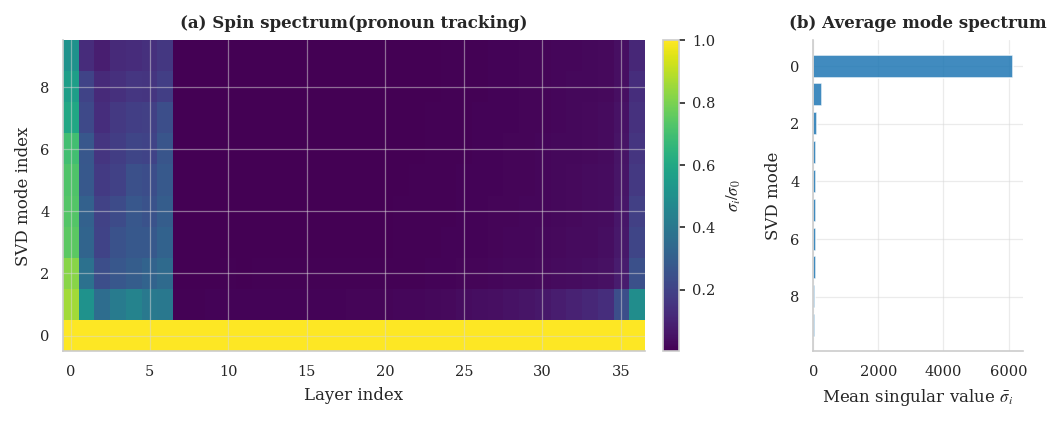
\includegraphics[width=\textwidth]{results_paper/Qwen3-4B-Base/spin_spectrum_(pronoun_tracking).png}
    \caption{Spin-spectrum view for \texttt{Qwen3-4B-Base}.}
\end{figure}

\begin{figure}[H]
    \centering
    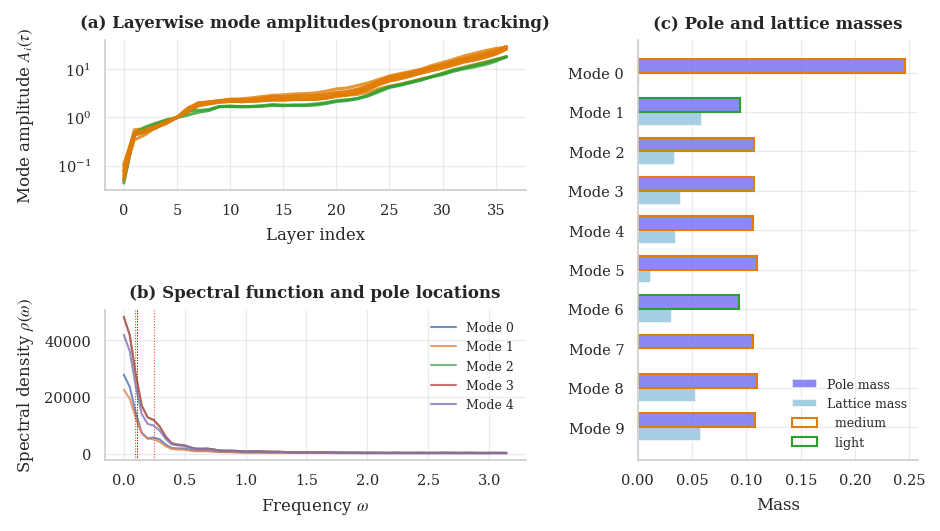
\includegraphics[width=\textwidth]{results_paper/Qwen3-4B-Base/mass_spectrum_(pronoun_tracking).png}
    \caption{Mass spectrum for \texttt{Qwen3-4B-Base}.}
\end{figure}

\begin{figure}[H]
    \centering
    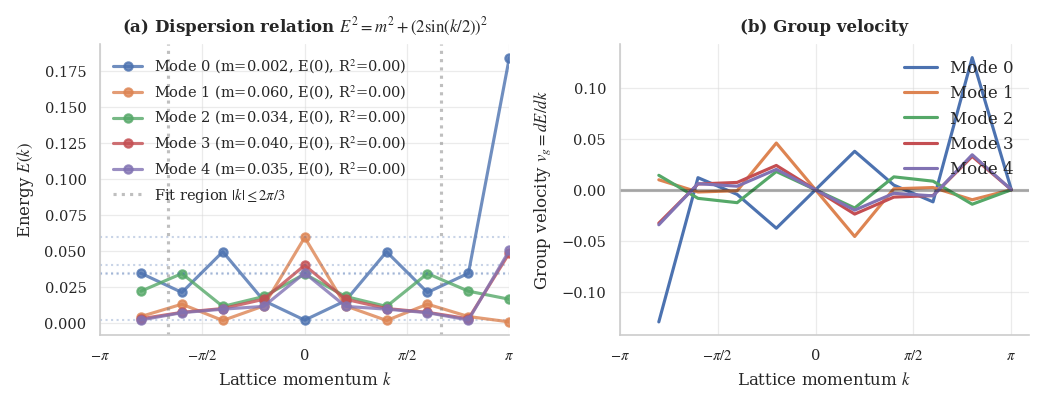
\includegraphics[width=\textwidth]{results_paper/Qwen3-4B-Base/dispersion_relation.png}
    \caption{Dispersion relation for \texttt{Qwen3-4B-Base}.}
\end{figure}

\begin{figure}[H]
    \centering
    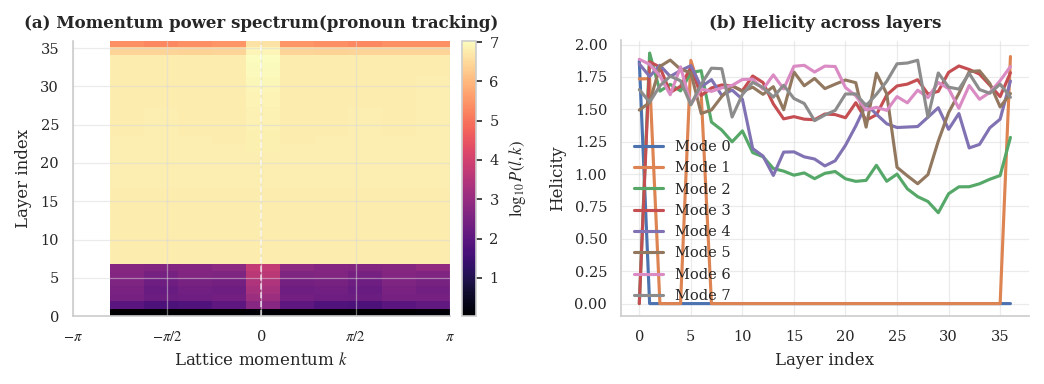
\includegraphics[width=\textwidth]{results_paper/Qwen3-4B-Base/momentum_helicity_(pronoun_tracking).png}
    \caption{Momentum-helicity summary for \texttt{Qwen3-4B-Base}.}
\end{figure}

\begin{figure}[H]
    \centering
    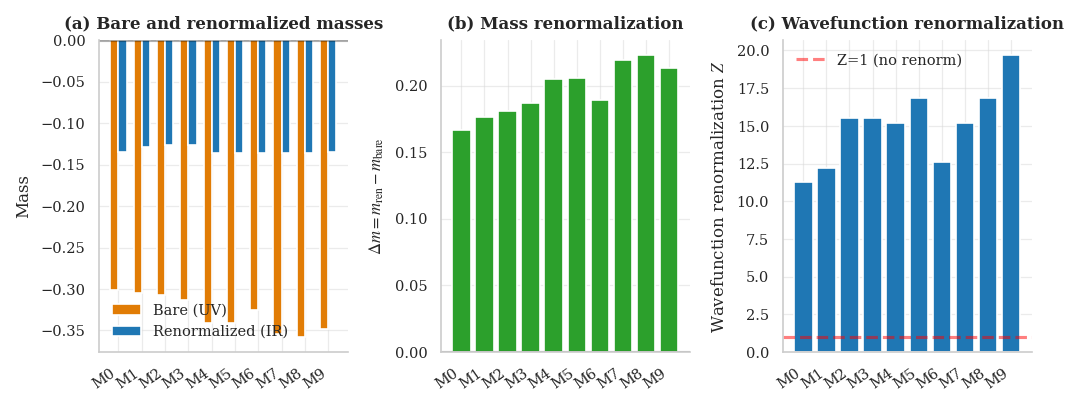
\includegraphics[width=\textwidth]{results_paper/Qwen3-4B-Base/eft_parameters.png}
    \caption{EFT parameter visualization for \texttt{Qwen3-4B-Base}.}
\end{figure}

\begin{figure}[H]
    \centering
    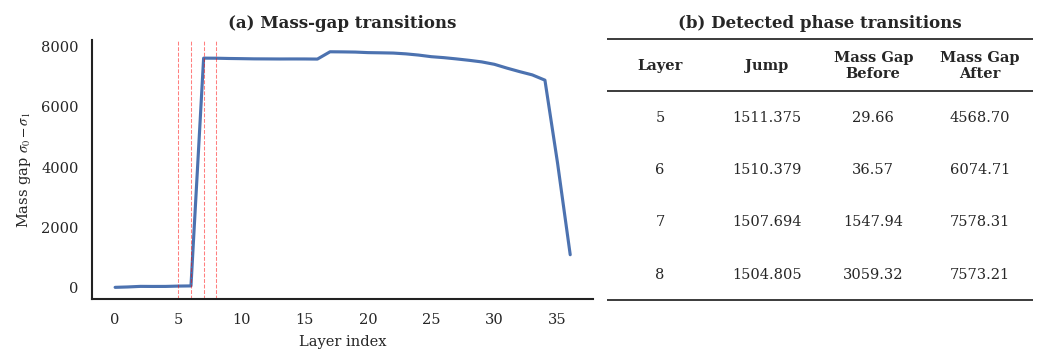
\includegraphics[width=\textwidth]{results_paper/Qwen3-4B-Base/phase_transitions.png}
    \caption{Phase-transition diagnostics for \texttt{Qwen3-4B-Base}.}
\end{figure}

\begin{figure}[H]
    \centering
    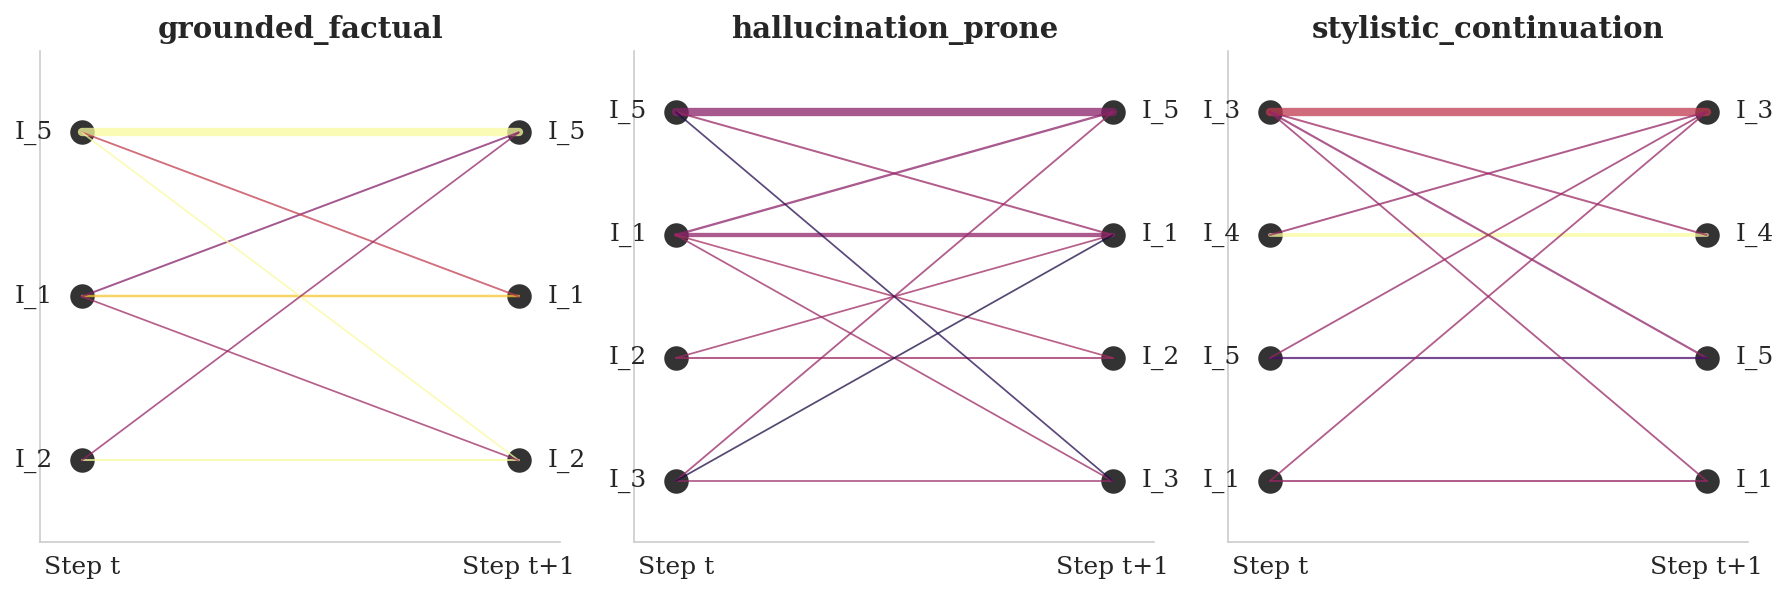
\includegraphics[width=\textwidth]{results_paper/Qwen3-4B-Base/intelliton_transition_graph.png}
    \caption{Species transition graph for \texttt{Qwen3-4B-Base}.}
\end{figure}

\section{Expanded cross-model figures}
\begin{figure}[H]
    \centering
    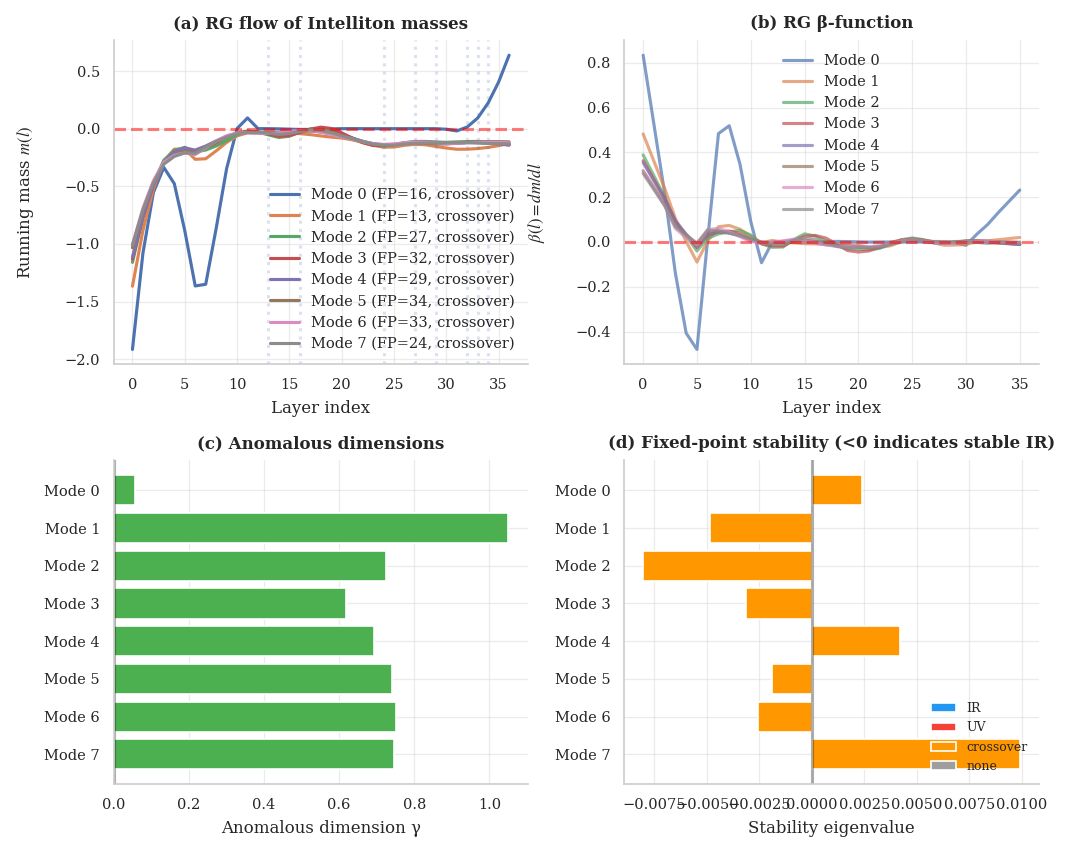
\includegraphics[width=\textwidth]{results_paper/Qwen3-4B/rg_flow.png}
    \caption{Appendix RG-flow diagnostics for \texttt{Qwen3-4B}.}
\end{figure}

\begin{figure}[H]
    \centering
    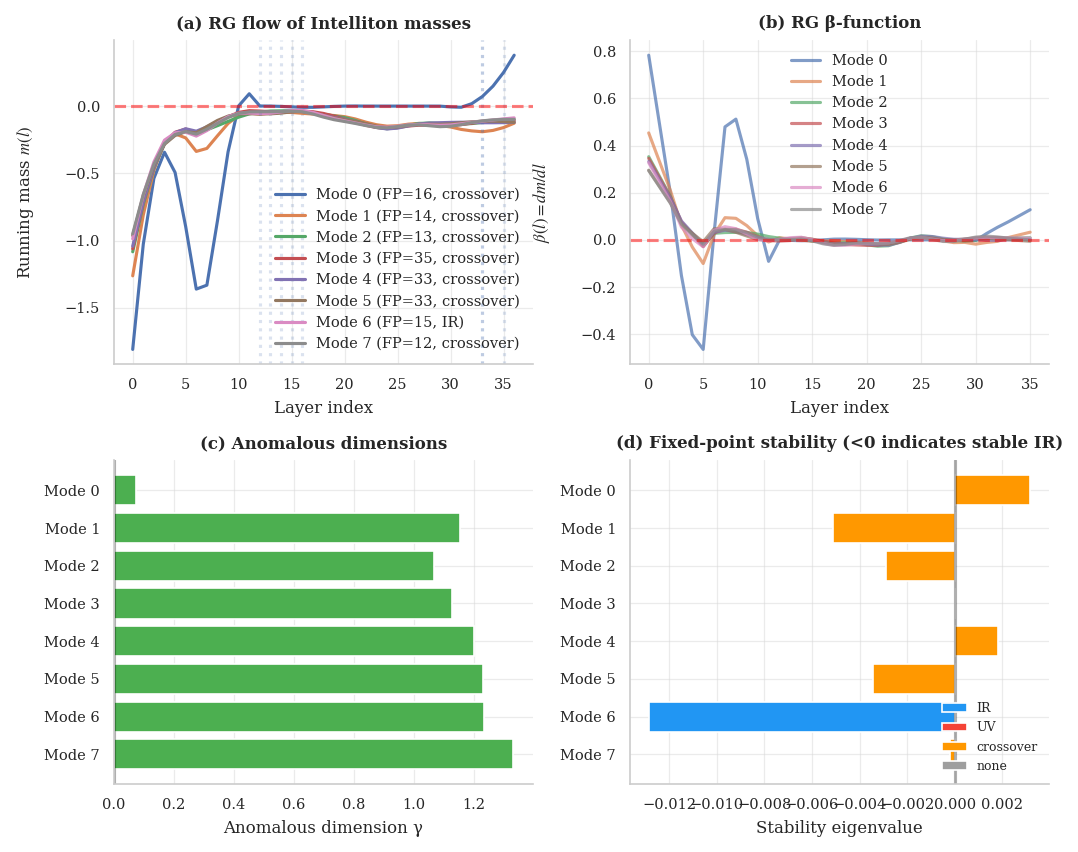
\includegraphics[width=\textwidth]{results_paper/Qwen3-8B/rg_flow.png}
    \caption{Appendix RG-flow diagnostics for \texttt{Qwen3-8B}.}
\end{figure}

\section{Compact quantitative comparison tables}
\begin{table}[H]
    \centering
    \caption{Model-level summary of Intelliton catalog size and grounded trajectory strength.}
    \label{tab:model-summary}
    \begin{tabular}{lccc}
        \toprule
        Model & Species count & Grounded activation mean & Grounded activation std \\
        \midrule
        Qwen3-4B-Base & 6 & 32.68 & 2.77 \\
        Qwen3-8B-Base & 7 & 60.26 & 4.67 \\
        Qwen3-4B & 5 & 29.13 & 5.77 \\
        Qwen3-8B & 6 & 57.14 & 4.68 \\
        Mistral-7B-v0.3 & 25 & 21.48 & 46.56 \\
        \bottomrule
    \end{tabular}
    \end{table}

\begin{table}[H]
    \centering
    \caption{Leading Intelliton species across models.}
    \label{tab:leading-species}
    \begin{tabular}{lcccccc}
        \toprule
        Model & Species & Spin & Mass(pole) & Momentum & FP layer & Amplitude \\
        \midrule
        Qwen3-4B-Base & $I_0$ & 1.84 & 0.1275 & 3.142 & 16 & 6167.1 \\
        Qwen3-8B-Base & $I_0$ & 1.74 & 0.1007 & 3.142 & 16 & 7908.4 \\
        Qwen3-4B & $I_0$ & 1.86 & 0.1281 & 1.885 & 16 & 6562.4 \\
        Qwen3-8B & $I_0$ & 1.78 & 0.1147 & 3.142 & 16 & 10080.2 \\
        Mistral-7B-v0.3 & $I_0$ & 1.98 & 0.1291 & 0.000 & 19 & 249.4 \\
        \bottomrule
    \end{tabular}
\end{table}

\section{Appendix catalog figures in landscape layout}
\begin{landscape}
\begin{figure}[p]
    \centering
    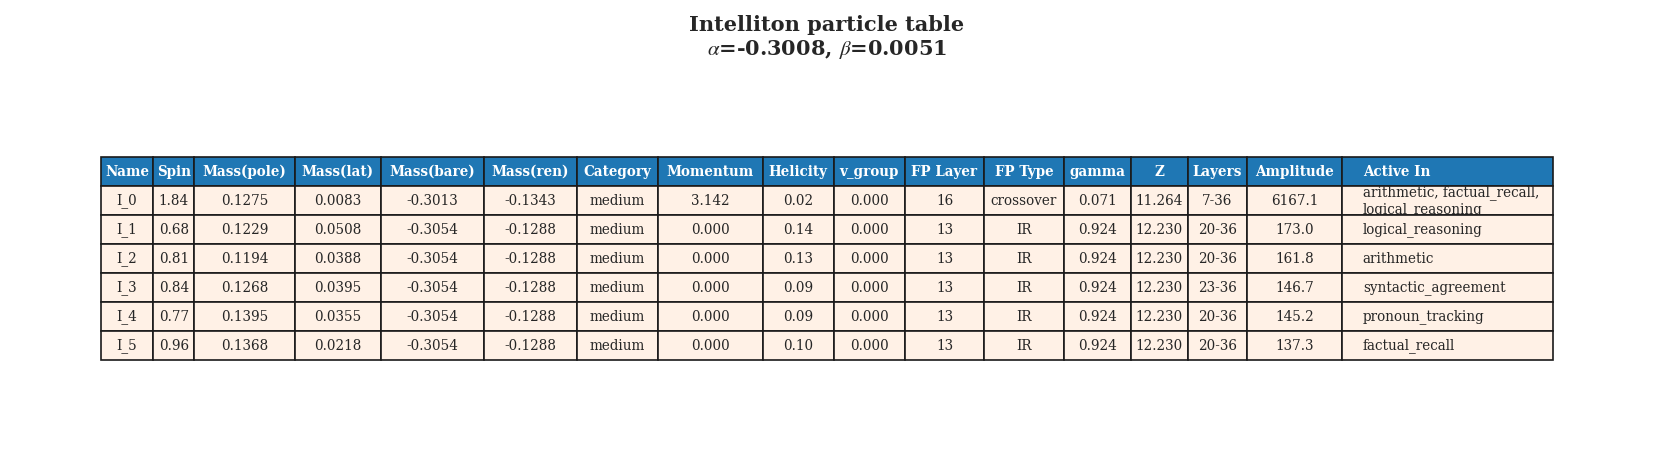
\includegraphics[width=\linewidth]{results_paper/Qwen3-4B-Base/particle_table.png}
    \caption{Independent Intelliton catalog figure for \texttt{Qwen3-4B-Base}.}
    \label{fig:appendix-qwen4bbase-catalog}
\end{figure}

\begin{figure}[p]
    \centering
    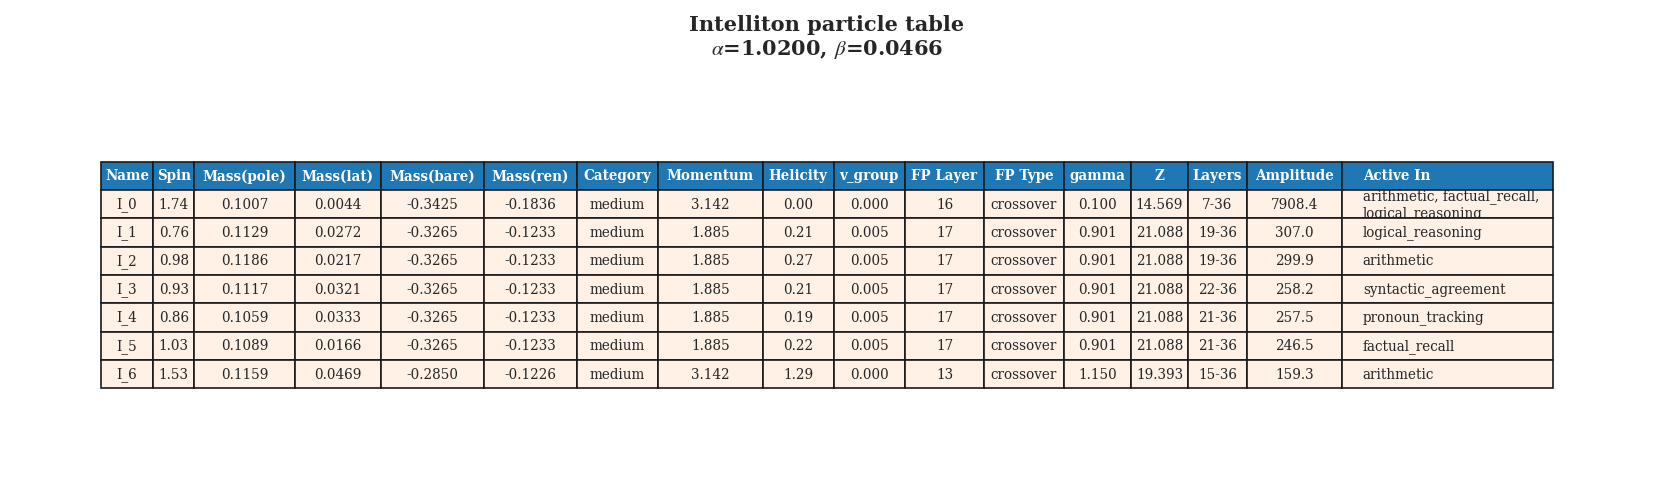
\includegraphics[width=\linewidth]{results_paper/Qwen3-8B-Base/particle_table.png}
    \caption{Independent Intelliton catalog figure for \texttt{Qwen3-8B-Base}.}
    \label{fig:appendix-qwen8bbase-catalog}
\end{figure}

\begin{figure}[p]
    \centering
    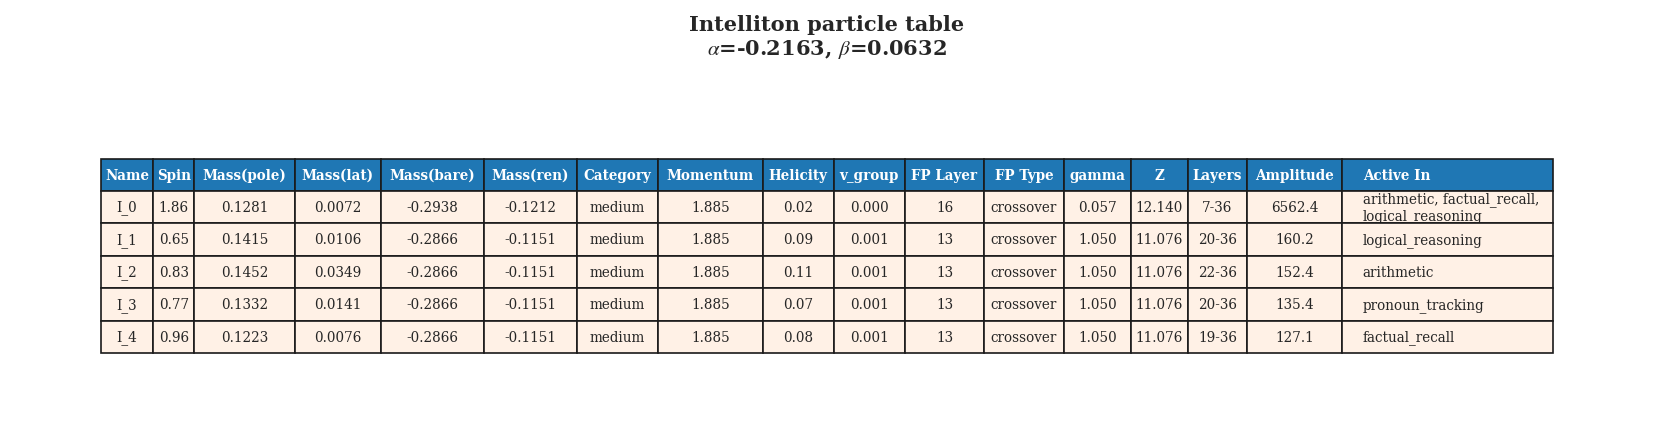
\includegraphics[width=\linewidth]{results_paper/Qwen3-4B/particle_table.png}
    \caption{Independent Intelliton catalog figure for \texttt{Qwen3-4B}.}
    \label{fig:appendix-qwen4b-catalog}
\end{figure}

\begin{figure}[p]
    \centering
    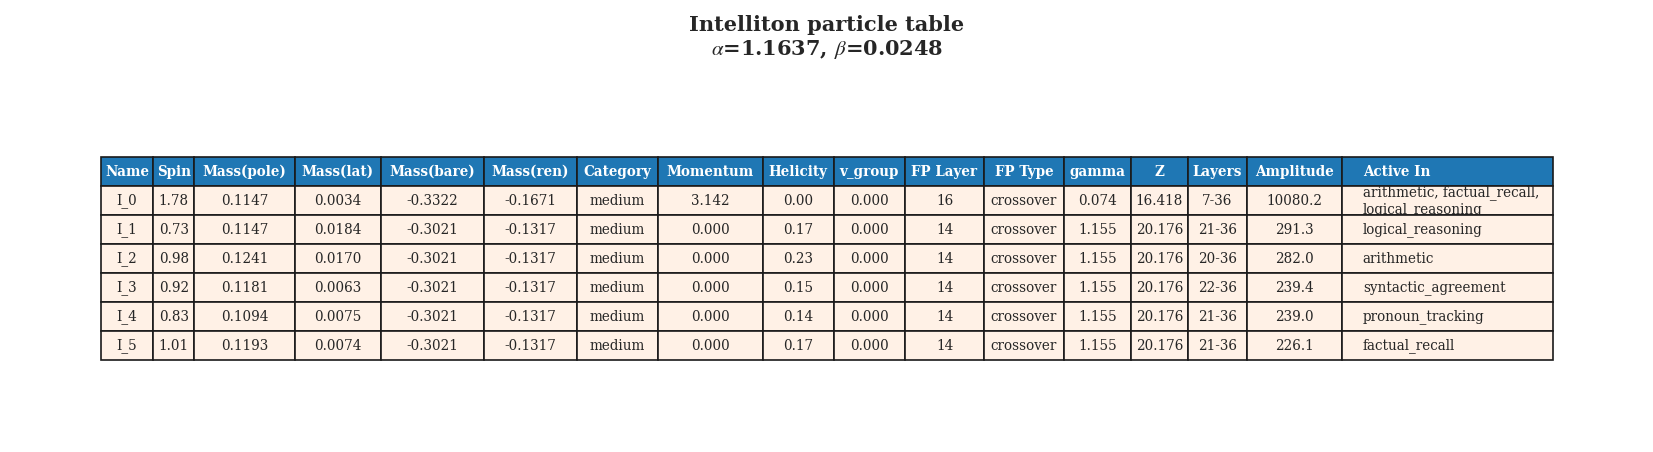
\includegraphics[width=\linewidth]{results_paper/Qwen3-8B/particle_table.png}
    \caption{Independent Intelliton catalog figure for \texttt{Qwen3-8B}.}
    \label{fig:appendix-qwen8b-catalog}
\end{figure}

\begin{figure}[p]
    \centering
    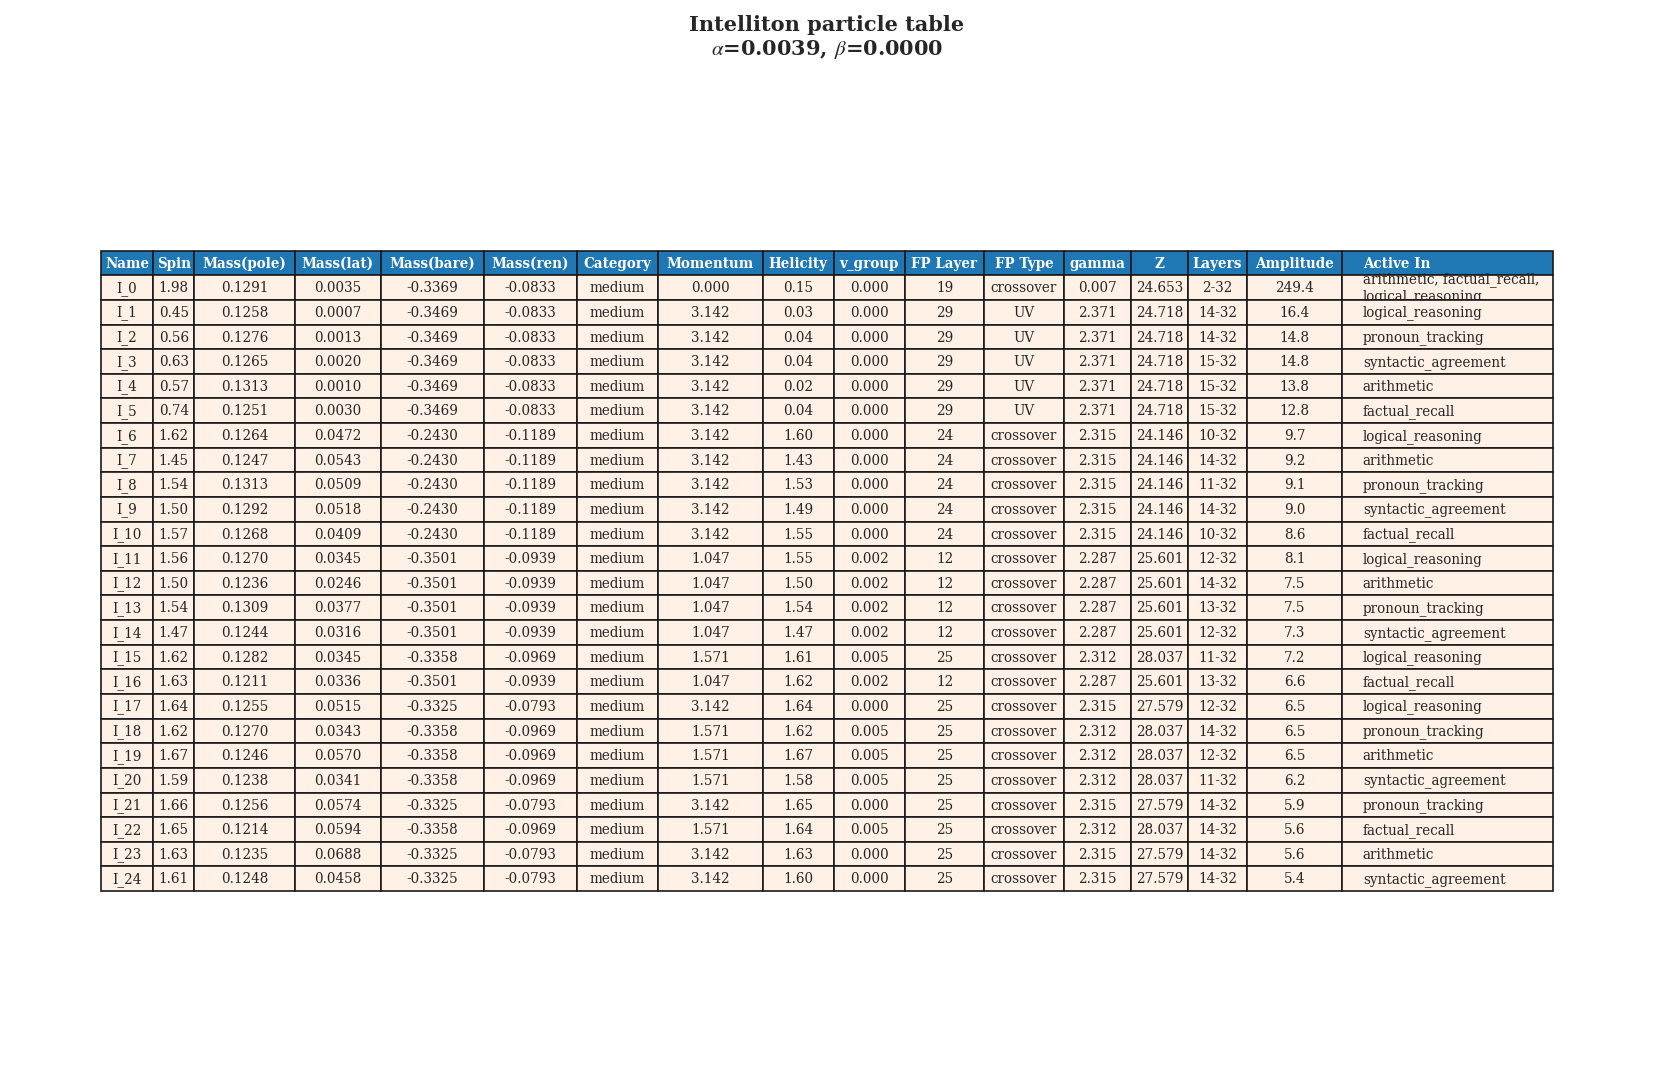
\includegraphics[width=\linewidth]{results_paper/Mistral-7B-v0.3/particle_table.png}
    \caption{Independent Intelliton catalog figure for \texttt{Mistral-7B-v0.3}.}
    \label{fig:appendix-mistral-catalog}
\end{figure}
\end{landscape}

\section{Notes on reproducibility}
The experiments are driven by \texttt{run\_paper.py}, which iterates over the canonical model list and executes the paper-oriented pipeline defined in \texttt{src/paper\_pipeline.py}. Core outputs include \texttt{intelliton\_catalog.csv}, \texttt{intelliton\_trajectory\_summary.csv}, \texttt{intelliton\_trajectory\_detail.csv}, \texttt{intelliton\_transition\_graph.csv}, and a standardized suite of per-model figures. The appendix catalog figures and summary tables in this paper were transcribed directly from those generated outputs.

\bibliographystyle{plainnat}
\bibliography{references}

\end{document}
